%%%%%%%%%%%%%%%%%%%%%%%%%%%%%%%%%%%%%%%%%%%%%%%%%%%%%%%%%%%%%%%%
%%%%%%%%%%%%% Experimental evaluation
%%%%%%%%%%%%%%%%%%%%%%%%%%%%%%%%%%%%%%%%%%%%%%%%%%%%%%%%%%%%%%%%
\begin{table*}[t!]
\begin{center}
\begin{tabular}{p{.65\textwidth}p{.32\textwidth}}
\hspace*{.4cm}
\begin{tabular}{|l||c|c||c|c|}
\hline
\multirow{3}{*}{} &\multicolumn{2}{c||}{Classification} & \multicolumn{2}{c|}{Speed}\\
                  &\multicolumn{2}{c||}{(mAP)} & \multicolumn{2}{c|}{(fps)}\\
\cline{2-5}
& MF (our) & DT~\cite{Wang12} & MF (our) & DT~\cite{Wang12}\\
\hline\hline
HOF               & 47.2\% & 52.9\% & 346.8 &  \\\hline
MBHx              & 49.0\% & 52.0\% & 330.3 &  \\\hline
MBHy              & 50.4\% & 56.1\% & 330.3 &  \\\hline
HOF+MBHx+MBHy     & 53.9\% & 58.9\% & 218.7 &  \\\hline
HOF+MBHx+MBHy+HOG & 56.2\% & 60.0\% & 168.4 & 1.2 \\\hline
\end{tabular}
&
\mbox{}\vspace{-.55cm}\newline
\hspace*{.2cm}
\begin{tabular}{|l|c|c|}
\hline
             & xvid  & x264  \\\hline
5000 kbit/s  & 58.9\% & 57.5\% \\\hline
1000 kbit/s   & 58.2\% & 57.4\% \\\hline
500 kbit/s   & 57.7\% & 57.1\% \\\hline
250 kbit/s   & 57.7\% & 57.0\% \\\hline
\end{tabular}
%

\end{tabular}
\mbox{}\vspace{.1cm}\\
\caption[Evaluation of action classification accuracy]{{\bf Left:} Evaluation of action classification accuracy and the speed of feature computation for Hollywood2 action recognition benchmark. The speed of feature computation is reported for video of spatial resolution $640\times480$ pixels. {\bf Right:} Evaluation of action recognition accuracy in Hollywood2 under the variation of video compression in terms of video codecs and compression bit-rates. The results are reported for MF descriptors in combination with FV encoding.\vspace{-.2cm}}
\label{tab:HWD2}
\end{center}
\end{table*}

%In this section we evaluate the proposed descriptor and descriptor encoding schemes on Hollywood2~\cite{Marszalek09} and UCF50~\cite{Reddy12} action recognition benchmarks and compare the speed and the recognition accuracy to the state of the art. We report classification results as mean average precision (mAP) for Hollywood2 and accuracy (Acc.) for UCF50. Processing speed is reported as frame-per-second (fps). We first evaluate the accuracy and the computational cost of proposed descriptor and compare it to the state-of-the-art method~\cite{Wang11}. The second part of the evaluation concerns the speed and accuracy of descriptor encoding.

In this section we evaluate the proposed descriptor and encoding schemes on Hollywood2~\cite{Marszalek09}, UCF50~\cite{Reddy12}, HMDB51~\cite{Kuehne11} and UT-Interaction~\cite{Ryoo10} action recognition benchmarks (see Figure~\ref{fig:datasets}) and compare the speed and accuracy of action recognition to recent methods~\cite{Feng13,Wang12,Yu10}. We follow standard evaluation setups and report mean average precision (mAP) for Hollywood2 and mean accuracy (acc) for UCF50, HMDB51 and UT-Interaction datasets. The processing speed is reported in frames-per-second (fps), run at a single-core Intel Xeon E5345 (2.33 GHz).

%In this series of experiments we adopt the standard bag-of-features action classification pipeline~\cite{Schuldt04} and represent each video clip by a $l_1$-normalized histogram of quantized local features. For each extracted type of descriptor we compute a vocabulary of 4000 visual words using k-means and assign all features to their nearest visual word centroids. Taking into account the space-time pyramid, we end up with $4\times24=96$ channels which we put in the SVM with multi-channel exponential $\chi^2$-kernel~\cite{Zhang07}.

To recognize actions we use SVM with multi-channel exponential $\chi^2$-kernel~\cite{Zhang07} together with histogram-based action representations. For Fisher vector and VLAD encodings we use linear SVMs.


\subsection{Descriptor evaluation}
%To assess the performance of motion information in compressed video representation, we first evaluate the performance of STIP features~\cite{Laptev08} where MPEG flow was obtained from DivX compression of Hollywood2 video samples and upscaled to the original video resolution. Results for one channel HOF descriptors in this setup gives 0.432 mAP compared to 0.458 mAP obtained for the original STIP implementation using Lucas-Kanade optical flow.

Table~\ref{tab:HWD2}~(Left) presents results of action recognition using the proposed MPEG flow (MF) features %described in Section~\ref{sec:CDdescriptor} 
compared to Dense Trajectories (DT) baseline~\cite{Wang12} using histogram encoding. For the full combination of four descriptors the performance of DT ($\sim$60.0\%) is approximately four per-cent higher compared to MF features ($\sim$56.2\%). When comparing the speed of feature extraction for both methods measured on videos with $640\times480$ pixels spatial resolution, our method achieves 168fps which is about 7 times faster than real-time and 140 times faster compared to~\cite{Wang12}. The speed measurements in this experiment include the time of feature computation as well as the time for video reading and decompression. Our method spends most of the time on the aggregation of histogram-based video descriptors using intergral space-time histograms. 
Compared to~\cite{Wang12} we save $\sim$66\% by avoiding OF computation, $\sim$4\% by sparser descriptor sampling and $\sim$29\% by the aggregation of sparse motion vectors. The run-time of our descriptor is, hence, $<$1\% of descriptor computation time in~\cite{Wang12}. Reducing the number of descriptor types increases the speed of our method to 347fps (14 times real time) at the cost of $<$4\% drop in mAP. 

DT features~\cite{Wang12} are computed along point tracks which is different to our features computed inside the fixed-size video patches. To identify the source of $\sim$4\% mAP drop of our method compared to~\cite{Wang12}, we simplify DT features by first approximating free-shape trajectories in DT features by constant velocity trajectories (DT V*). In the second simplification we remove trajectory information from DT descriptor and compute DT features in fixed axes-parallel cuboids (DT V0). The results of these modifications in the first two lines of Table~\ref{tab:HWD2traj} indicate 1\% drop due to DT V* and 1\% further drop in mAP due to DT V0. Explicitly including the shape of trajectories into the descriptor (last line of Table~\ref{tab:HWD2traj}) does not improve performance significantly. From this experiment we conclude that the shape of trajectories does not contribute to other descriptors significantly. We believe that the difference in accuracy of DT features and our method should be in the denser and more accurate flow estimation deployed by DT. Per-class action classification comparison of MF and DT features is illustrated in Figure~\ref{fig:hwd2-barplot}.

\begin{table}
\begin{center}
\begin{tabular}{|l|c|c|}
\hline
& mAP \\\hline
HOF+MBHx+MBHy+HOG (V0)  					& 58.0\%	\\\hline
HOF+MBHx+MBHy+HOG (V*)						& 58.9\%	\\\hline
HOF+MBHx+MBHy+HOG \cite{Wang12}     	& 60.0\% 	\\\hline
HOF+MBHX+MBHY+HOG+TRAJ \cite{Wang12} 	& 60.3\% 	\\\hline
\end{tabular}
\mbox{}\vspace{.2cm}\\
\caption[Action classification accuracy]{Action classification accuracy on Hollywood2 dataset for different versions of the dense trajectory features~\cite{Wang12} in combination with histogram encoding}
\label{tab:HWD2traj}
\end{center}
\end{table}



\subsection{Descriptor encoding evaluation}
\label{subsec:descencimprov}
While our method achieves high speed descriptor computation, the feature quantization becomes a bottle-neck with nearest-neighbor (NN) quantization performing only at the rate of 10fps when using efficient $l_2$-distance implementation. To improve quantization speed, we experiment with tree-based approximate nearest neighbor (ANN) quantization schemes implemented in FLANN~\cite{Muja09}. The trade-off between computational time and the accuracy of quantization measured on the final recognition task is illustrated in Figure~\ref{fig:hwd2-flann}. Notably, the quantization using four trees and 32 tests in ANN search does not degrade recognition performance and achieves factor $\approx$ 5x speed-up compared to NN. Further increase of the speed implies approximately linear degradation of classification accuracy. 

We next investigated Fisher Vector (FV)~\cite{Perronnin12} and VLAD encodings~\cite{Jegou10} described in Section~\ref{sec:quantization}. 
%FV and VLAD representations have been shown to achieve high accuracy for image classification tasks~\cite{Chatfield11} and usually require smaller vocabularies compared to histogram encodings.
%
%Fisher vector and VLAD schemes are described in Section~\ref{sec:quantization}. 
The VLAD encoding has already been applied to action reconition in \cite{Jain13}, but here we also evaluate the full Fisher vector. We train a GMM model with $K=256$ Gaussians \cite{Jegou12}. Results in Figure~\ref{fig:hwd2-flann} and Table~\ref{tab:hwd2_comparison} indicate improvements in both the speed and accuracy when using FV and VLAD encodings compared to the histogram encoding. As for the histogram encoding, FLANN provides considerable speed-up for FV and VLAD encodings.

Table~\ref{tab:ucf_comparison} presents action recognition results for the UCF50 dataset. Similar to the Hollywood2 dataset, the accuracy of our methods is only a few percent below the state-of-the-art results in~\cite{Wang12} with FV and VLAD encodings providing improvements over the histogram encoding both in speed and accuracy. The overall speed improves the speed of~\cite{Wang12} by two orders of magnitude. Table~\ref{tab:uti_comparison} presents results for the UT-Interaction dataset and compares our method with the efficient action recognition method~\cite{Yu10}. Our method demonstrates better classification accuracy compared to~\cite{Yu10} and improves the speed of~\cite{Yu10} by one order of magnitude. %the factor of $10$.

In Table~\ref{tab:hmdb_comparison} we compare our results on the HMDB dataset to~\cite{Feng13} that investigates the effect of feature sampling on the trade-off between computational efficiency and recognition performance. For the MBH descriptor our method obtains significant improvement both in speed and accuracy, despite the fact that in~\cite{Feng13} the system was evaluated on Intel i7-3770K (3.50 GHz) which runs 1GHz faster than our Intel Xeon E5345 (2.33 GHz). Both systems were evaluated on a single core with no multithreading.

%Our Fisher vector implementation attributes a descriptor only to 5 nearest mixture centroids in $l_2$-sense in contrast to \cite{Jegou12} which fully computes $q_{ki}$ to all mixture centroids in their public implementation in the YAEL library\footnote{\scriptsize \url{https://gforge.inria.fr/projects/yael/}}. To make it faster we compute only the 5 nearest neighbors using kd-trees. Differently from YAEL we explicitly tailor our implementation to efficiently compute Fisher vector for several spatio-temporal grids. In addition, we found that the second order part $\textbf{v}_k$ (\ref{eq:fv_vk}) does not bring improvement, and we don't compute it.

%We also experiment with the VLAD representation that we get if we consider only one nearest neighbor during the process described above. With both representations we try different values for the number of tests performed during the descent down the kd-trees.

Recently, the method in \cite{Wang12} has been further improved using motion stabilization~\cite{Jain13,Wang13} and feature extraction from person tracks~\cite{Wang13}. These extensions are complementary to our work and can be used to improve results of our method.
%The authors also use Fisher vectors but without space-time binning. The accuracy is significantly higher than in \cite{Wang12} ($64.3\%$ on Hollywood2, $57.2\%$ on HMDB51 and $91.2\%$ for UCF50), but the speed is roughly the same. We consider the lower sparsity of optical flow and low number of descriptors per frame to be the main source of decreased accuracy of our method (see Table~\ref{tab:HWD2traj} (V0) compared to Table~\ref{tab:HWD2}). However, in need of very efficient action recognition the trade-off may be worth it. We consider the extensions of~\cite{Wang13} may be implemented in our method as well, but the efficiency will need to be studied.


\begin{table}
\begin{center}
\vspace{-.1cm}
\begin{tabular}{r|c|c|c|c|}
\cline{2-5}
& \multicolumn{2}{c|}{Farneback flow} & \multicolumn{2}{c|}{MPEG flow} \\\hline
\multicolumn{1}{|r|}{Sampling stride} & mAP & fps & mAP & fps \\\hline
\multicolumn{1}{|r|}{16}  	& 58.3\% & 35.2	& 58.2\% & 168.4\\\hline
\multicolumn{1}{|r|}{8}   	& 58.6\% & 24.1 & &	\\\hline
\multicolumn{1}{|r|}{4}     	& 59.2\% & 13.7	& &     \\\hline
\end{tabular}
\mbox{}\vspace{.2cm}\\
\caption[Action classification accuracy on Hollywood2 dataset]{Action classification accuracy on Hollywood2 dataset using sparse sampling of Farneback flow and MPEG flow followed by FV feature encoding. The reported speed of feature extraction is affected by the increased computational cost of aggregating motion vectors into local descriptors. \vspace{-.6cm}}
\label{tab:flow_resample}
\end{center}
\end{table}



\subsection{Parameter sensitivity}
MPEG flow might be influenced by the types and parameters of video codecs. To investigate this aspect, we evaluate the performance of action recognition for two common video codecs (x264 and xvid) under varying video compression bit-rates. Results in Table~\ref{tab:HWD2} (Right) indicate the stable performance of action recognition for different types of video codecs and decreasing video quality corresponding to low values of bit-rates. 

We have also evaluated the influence of sparse flow sampling on the speed and accuracy of action recognition. In Table~\ref{tab:flow_resample} we illustrate accuracy of our method when using Farneback flow and MPEG flow. Denser flow sampling (Farneback) leads to slight improvements in recognition accuracy by the cost of significantly increased computation time. Notably, sparse Farneback and MPEG flow show similar recognition performance.

\begin{figure}
\begin{center}
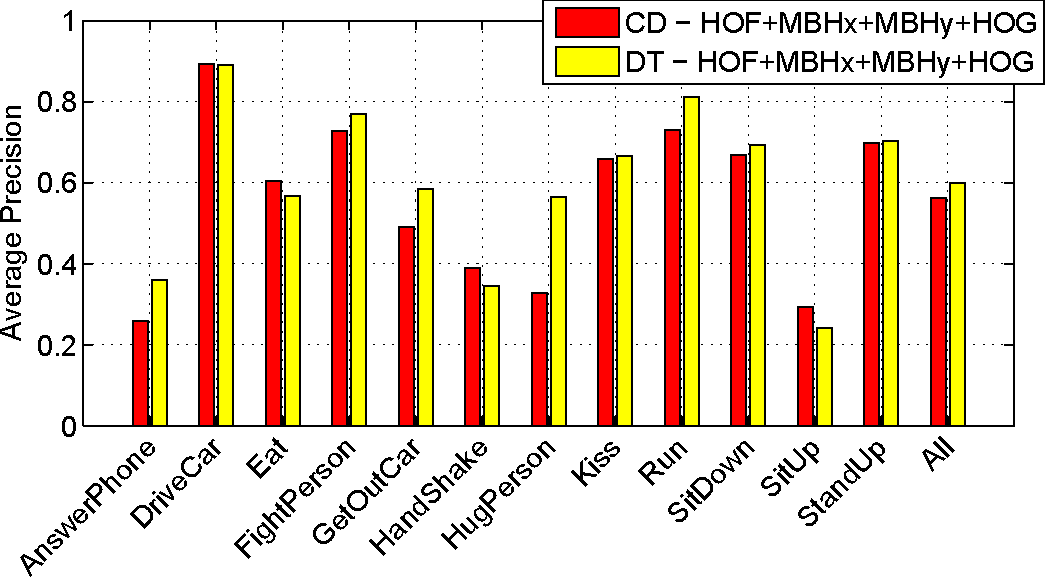
\includegraphics[width=.9\linewidth]{cvpr14_figures/hollywood2-per-class-barplot-crop.pdf}.
\caption[Per-class action classification results]{Per-class action classification results for DT~\cite{Wang12} and our  MF features using HOF+MBHx+MBHy+HOG descriptor combination and histogram encoding on the Hollywood2 benchmark.\vspace{-.1cm}}
\label{fig:hwd2-barplot}
\end{center}
\end{figure}

\begin{figure}
\begin{center}
\mbox{}\vspace{-.4cm}\\
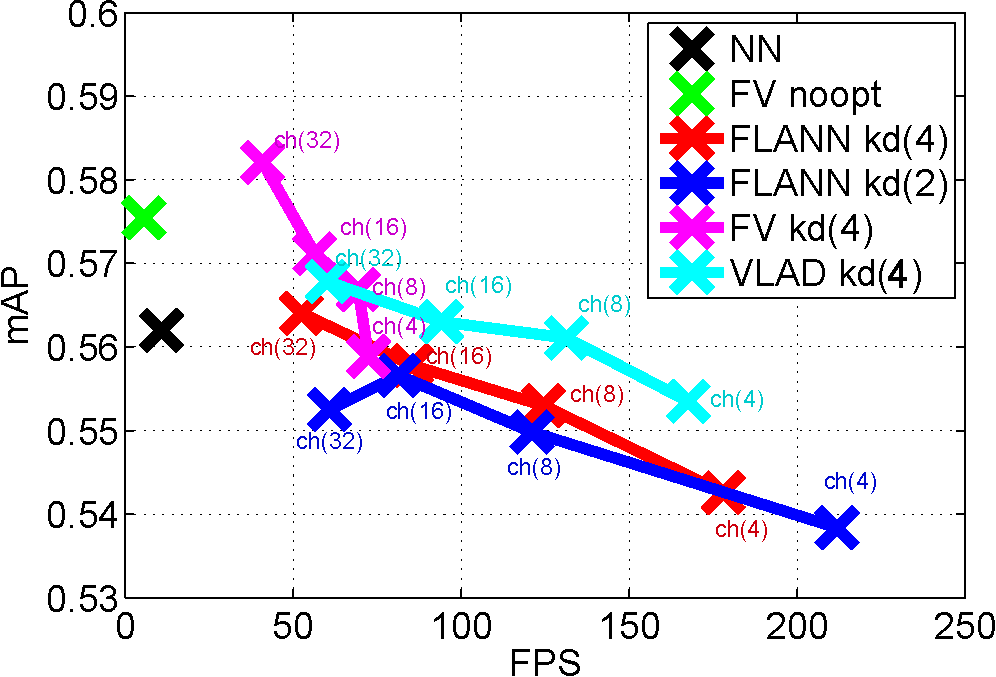
\includegraphics[width=.9\linewidth]{cvpr14_figures/hollywood2-flann-fps-map-crop-mod.pdf}
\caption[Performance of action recognition]{Performance of action recognition and the speed of descriptor encodings in Hollywood2 dataset for different types and parameters of encoding schemes. kd($x$) indicates the number of trees $x$ in the kd-forest used for ANN descriptor assignment. ch($y$) indicates the number of tests $y$ when descending the forest.\vspace{-.4cm}}
\label{fig:hwd2-flann}
\end{center}
\end{figure}




\begin{table}
\begin{center}
\begin{tabular}{|l|c|c|c|c|}
\hline
		 				&  	 		& Feat.                   	& Quant. 		& Total		\\
		 				& Acc.  	& (fps)								& (fps)			& (fps)		\\\hline
MF FLANN(4-32)	& 55.8\%	& \multirow{3}{*}{168.4} 	& 52.4    	& 40.0 	\\ % FPS = 1/(1/168.4 + 1/52.3921)
MF VLAD(4) 		& 56.7\%	&										& 167.5	& 84.0	\\ % FPS = 1/(1/168.4 + 1/167.537313)
MF FV(32)			& 58.2\%	&										& 40.9 	& 32.9	\\ % FPS = 1/(1/168.4 + 1/40.8925322)
\hline
DT \cite{Wang12}& 59.9\%		& 1.2									& 5.1 		&	1.0	\\\hline % Quant. FPS = 1346 frames / 266.17 secs = 5.0569 FPS; Total = 1/(1/1.2 + 1/5.0569) = 0.9699 FPS
%\cite{le_at_al}						& 53.3\%		&										&				&\\\hline
\end{tabular}
\mbox{}\\
\caption[Comparison of our method to the state of the art on Hollywood2 dataset]{Comparison of our method to the state of the art on Hollywood2 dataset. The speed of~\cite{Wang12} and of our method is reported for videos with spatial resolution $640\times 480$ pixels.\vspace{-.3cm}}
\label{tab:hwd2_comparison}
\end{center}
\end{table}



\begin{table}
\begin{center}
\begin{tabular}{|l|c|c|c|c|}
\hline
		 				&  	 	& Feat.                    & Quant. 	& Total	\\
		 				& Acc.  & (fps)                    & (fps) 	& (fps)	\\\hline
MF FLANN(4-32)	& 81.6\% & \multirow{3}{*}{591.8}   & 52.4  	& 48.1	\\ % FPS = 1/(1/592 + 1/52.3921)
MF VLAD(4) 	 	& 80.6\% &                          & 671.4 	& 314.6	\\ % FPS = 1/(1/592 + 1/671.428571)
MF FV(32)	 		& 82.2\% &                          & 171.3 	& 132.8	\\ % FPS = 1/(1/592 + 1/171.255061)
\hline
DT \cite{Wang12}& 85.6\% & 2.8            	        & 5.1  	& 1.8\\\hline%  Feat extr FPS = 846 frames / 5m; Quant FPS = 846 frames / 166.17 secs = 5.0912 FPS; Total = 1 / (1/2.8 + 1/5.0912) = 1.8065 FPS
%\cite{Kliper12}		&	72.7\%	&									&			&\\\hline
\end{tabular}
\smallskip
\caption[Comparison of our method to the state of the art on the UCF50 dataset]{Comparison of our method to the state of the art on the UCF50 dataset~\cite{Reddy12}. The speed is reported for videos with the spatial resolution $320\times 240$ pixels.}
\label{tab:ucf_comparison}
\mbox{}\vspace{-1cm}\\
\end{center}
\end{table}


\begin{table}
\begin{center}
\begin{tabular}{|l|c|c|}
% set1_segmented
%   sample acc = 85.238095
%   feat extr fps = 7280 frames / 15.990000 sec = 455.2846 fps
%	 quant time fps = 7280 frames / 61.720000 = 117.9520 fps
%   total_fps = 1 / (1/455.2846 + 1/117.9520) = 93.6816 fps
% set2_segmented
%	 sample acc = 87.6190
% 	 feat extr fps = 6515 frames / 12.160000 sec = 535.7730 fps
%   quant time fps = 6515 frames / 50.100000 = 130.0399fps
%   total_fps = 1 / (1/535.7730 + 1/130.0399) = 104.6418
% average fps: (93.6816 + 104.6418)/2 = 99.1617
% average acc: (85.238095 + 90.000000) / 2 = 87.6190
\hline
								& Acc.		& Total FPS	\\\hline
FV(32)						& 87.6\%		& 99.2		\\\hline
PSRM+BOST\cite{Yu10}	& 83.3\%		& 10.0 		\\\hline

\end{tabular}
\mbox{}\vspace{.2cm}\\
\caption[Accuracy and speed of action recognition]{Accuracy and speed of action recognition in the UT-interaction dataset~\cite{Ryoo10}.\vspace{-.6cm}}
\label{tab:uti_comparison}
\end{center}
\end{table}

\begin{table}
\begin{center}
\begin{tabular}{|l|c|c|c|c|}
\hline
% for KnifeThrowingJackDaggerDemoReel_throw_f_nm_np1_fr_med_2.avi (410 frames, 360x240)
		 				&  	 		& Feat.                    & Quant. 	& Total	\\
		 				& Acc.		& (fps)                    & (fps) 	& (fps)	\\\hline
MF ALL FV(32)		& 46.7\% 	& 455.6                    & 129.7 	& 101.0	\\ % FPS = 410 / 0.9 = 455.5556, 410 / 3.16 = 129.7468, 1 / (1/455.5556 + 1/129.7468) =   101.0
MF MBH FV(32)		& 45.4\% 	& 683.3                    & 268.0 	& 192.5	\\ % FPS = 410 / 0.6 = 683.3333, 410 / 1.53 = 267.9739, 1 / (1/683.3333 + 1/267.9739) =   192.4883
MF ALL VLAD(32) & 46.3\%	& 455.6								& 455.6		& 227.8	\\ % FPS = 410 / 0.9 = 455.5556, 1 / (1/455.5556 + 1/455.5556) =   227.7778
\hline
MBH \cite{Feng13}		& 41.1\% 	& 33.9            	     	& 267.1 & 30.8	\\ % FPS = 1/(1/41.19 + 1/192.4) = 33.9268
HOG3D \cite{Feng13}	& 33.3\% 	& 49.6            	   	& 290.8 & 42.2	\\ % FPS = 1/(1/71.88 + 1/159.60)= 49.5596
%Combined \cite{Feng13} & 47.6\% & 									&			&			\\
DT	\cite{Wang12}			& 48.3\%& 3.1								&			& \\ % FPS = 410 / 133.26 = 3.0767
\hline
\end{tabular}
\smallskip
\caption[Comparison of our method to \cite{Feng13} on the HMDB dataset~\cite{Kuehne11}]{Comparison of our method to \cite{Feng13} on the HMDB dataset~\cite{Kuehne11}. The speed is reported for videos with the spatial resolution $360\times 240$ pixels}
\label{tab:hmdb_comparison}
\mbox{}\vspace{-1cm}\\
\end{center}
\end{table}

%Hollywood2 results (A): Compressed domain features
%HOF: 0.472243
%MBHx: 0.490259
%MBHy: 0.503737
%HOF+MBHx+MBHy: 0.539212
%HOF+MBHx+MBHy+HOG (m/channel): 0.561959
%HOF+MBHx+MBHy+HOG (single vocab): 0.517230

%Hollywood2 results (B): Dense trajectory features
%HOF : 0.528732
%MBHX : 0.519922
%MBHY : 0.561268
%HOF_MBHX_MBHY : 0.589344
%HOF_MBHX_MBHY_HOG : 0.599716
%HOF_MBHX_MBHY_TRAJ : 0.591272
%HOF_MBHX_MBHY_HOG_TRAJ: 0.603235

%HOG+HOF+MBHx+MBHy:
%VEL0: 0.580140
%FST: 0.589389

%Hollywood2 results (C): Compressed domain features + FLANN; 
%HOF: 0.480621
%MBHx: 0.480726
%MBHy: 0.499320
%HOF+MBHx+MBHy: 0.540788
%HOF_MBHx_MBHy_HOG (m/channel): 0.564032

% per-class results in 
% https://docs.google.com/spreadsheet/ccc?key=0Al7q11u9-vugdDk4UlhrWjVxNm5Ldk9EMjVEZTZVM0E&pli=1#gid=0
% D:\doc\papers\descriptors\cvpr13\results\Class. results by class.xlsx

%%%%%%%%%%% computation time, election video 1800 frames 120 sec. 15fps (-> 72sec at 25fps)
% CD features   10.69 sec ->  168.3817 fps
% HOF only:     5.19 sec -> 346.8 fps
% MBHx 0nly:    5.45 sec -> 330.3 fps
% HOF+MBHx+MBHy 8.23 sec -> 218.7 fps
%
%# STAT. Descriptor computation: 3.13 secs
%# STAT. HOF: 0.42, MBH: 1.49 secs, HOG: 0.71 secs
%# STAT. Interpolation. HOFMBH: 0.14 secs, HOG: 0.37 secs
%# STAT. Descriptor querying: 3.60 secs
%# STAT. HOF: 0.84, MBH: 1.55 secs, HOG: 0.79 secs
%# STAT. Reading: 0.04 secs
%# STAT. Decoding: 3.75 secs
%# STAT. Writing: 87.96 secs
%# STAT. ---
%# STAT. Total: 98.65 secs
%# STAT. fps: 18.24
%# STAT. calls:
%# STAT. --ComputeDescriptor     6467808
%
% DT features: 24m56sec -> 1.2032 fps
%
% CD vs. DT speedup: x139.9449

%%%%%%%%%%% computation time, actioncliptest00775 1347 frames, 53.8 sec.
% CD features 9.35 sec -> 144.0642 fps
%# STAT. Descriptor computation: 2.79 secs
%# STAT. HOF: 0.29, MBH: 1.28 secs, HOG: 0.85 secs
%# STAT. Interpolation. HOFMBH: 0.07 secs, HOG: 0.30 secs
%# STAT. Descriptor querying: 3.22 secs
%# STAT. HOF: 1.00, MBH: 1.27 secs, HOG: 0.61 secs
%# STAT. Reading: 0.04 secs
%# STAT. Decoding: 3.00 secs
%# STAT. Writing: 71.45 secs
%# STAT. ---
%# STAT. Total: 80.80 secs
%# STAT. fps: 16.67
%# STAT. calls:
%# STAT. --ComputeDescriptor     4596504
%
% DT features 28m37sec -> 0.7845 fps
% real    28m37.449s
% user    28m26.158s
% sys     0m13.664s
%
% CD vs. DT speedup: x183.6382



% Quantization for actioncliptest00775 1347 frames, 53.8 sec.
%
%
% kd(8) + checks(32) 38.90 secs ->  34.6272      mAP 0.563959
% kd(8) + checks(16) 23.56 secs ->  57.1732      mAP 0.560811
% kd(8) + checks(8)  13.18 secs -> 102.2003      mAP 0.553482
% kd(8) + checks(4)  11.52 secs -> 116.9271      mAP 0.526568

% kd(4) + checks(32) 25.71 secs ->  52.3921 fps (mAP 0.564032)

% kd(4) + checks(16) 15.80 secs ->  85.2532     (mAP 0.557820)
% kd(4) + checks(8)  10.82 secs -> 124.4917     (mAP 0.552988)
% kd(4) + checks(4)   7.57 secs -> 177.9392     (mAP 0.542571)
% kd(2) + checks(32) 22.17 secs ->  60.7578     (mAP 0.552528)
% kd(2) + checks(16) 16.56 secs ->  81.3406     (mAP 0.556588)
% kd(2) + checks(8)  11.13 secs -> 121.0243     (mAP 0.549832)
% kd(2) + checks(4)   6.36 secs -> 211.7925     (mAP 0.538391)
%
%

%Quantization for actioncliptest00775 1347 frames, regular FV, just mu params
%Options:
%Indices are zero-based
%213-308 '../../vocab/mbhx_K256.vocab'
%Build GMM index: no
%GMM components: 256
%Lambda reg: 0.000000
%Output file path: out.npy
%Zero all gamma but: 0
%XnPos: 0, YnPos: 1, TnPos: 2
%Grids: 1x1x1x
%Vocabularies loaded
%
%#FV 1x1x1x  mbhx_K256 (213-308)
%fts.cols: 96
%24576
%No zeroing
%24576
%# 0-0-0 (380014)
%#STAT Vocab reading and construction: 0.03 secs
%#STAT Reading: 21.32 secs
%#STAT Writing: 0.00 secs
%#STAT Assigning: 164.76 secs
%#STAT Copying: 0.41 secs
%#STAT Total: 186.54 secs
%#STAT Ops: 1
%#STAT Descriptors: 380014
%#STAT Part sizes: 96

% Quantization for actioncliptest00775 w=640	h=480	frames=1347.00
%KNN_TREES_CHECKS FLANN ASSIGNING TOTAL FPS
%5_4_32 22.870000 10.070000 32.940000 40.892532		mAP 0.582075 (c =1e-3)
%5_4_16 13.890000 9.990000 23.880000 56.407035		mAP 0.571156 (c=1)
%5_4_8 9.000000 10.430000 19.430000 69.325785		mAP 0.566866 (c=1)
%5_4_4 6.720000 11.880000 18.600000 72.419355		mAP 0.558892 (c=1)

%1_4_32 19.780000 2.650000 22.430000 60.053500		mAP 0.567833 (c=1)
%1_4_16 11.580000 2.730000 14.310000 94.129979		mAP 0.563006 (c=0.1-1)
%1_4_8 7.540000 2.720000 10.260000 131.286550		mAP 0.561079 (c=1)
%1_4_4 5.300000 2.740000 8.040000 167.537313			mAP 0.553502 (c=1)

%3_4_32  21.350000       6.300000        27.650000       48.716094 mAP 0.565615 (c=1)
%3_4_16 mAP 0.562545 (c=1e-1)
%3_4_8 mAP 0.565996 (c=1)
%3_4_4   5.730000        6.760000        12.490000       107.846277 mAP 0.558180 (c=1)



%UCF50 w=320	h=240 frames=846.00 v_Rowing_g15_c05.avi  ; #features: 48944 => 57.8 features / frame
%5_4_32  3.350000        1.590000        4.940000        171.255061
%1_4_4   0.810000        0.450000        1.260000        671.428571
% feature extraction:  1.4200 => 595.7746 fps
%5_4_32 => total fps: 132.8761
%1_4_4  => total fps: 315.6401


%HMDB51 w=320 h=240	frames=75.0 Iaido_video_instruction_series_Wehrhahn_Sensei_sword_exercise_f_nm_np1_le_bad_1.avi  ; #features: 3864 => 51.5 features / frame
%5_4_32  0.300000        0.110000        0.410000        182.926829
%1_4_4   0.060000        0.040000        0.100000        750.000000
% feature extraction: 0.18sec => 416.6667 fps
%5_4_32 => total fps: 127.0918
%1_4_4  => total fps: 267.5815

%UCF50 extr. time on v_Rowing_g15_c05.avi. !! DescrComp + Interp + DescrQue + Reading + Decoding: 1.43 sec, 846 frames => 592 fps 
%# STAT. Descriptor computation: 0.47 secs
%# STAT. HOF: 0.05, MBH: 0.21 secs, HOG: 0.15 secs
%# STAT. Interpolation. HOFMBH: 0.01 secs, HOG: 0.05 secs
%# STAT. Descriptor querying: 0.55 secs
%# STAT. HOF: 0.13, MBH: 0.25 secs, HOG: 0.07 secs
%# STAT. Reading: 0.01 secs
%# STAT. Decoding: 0.34 secs
%# STAT. Writing: 8.97 secs


